\begin{landscape}
\section{Domainmodel}
	Im folgenden Diagramm sind die wichtigsten konzeptionellen Klassen und ihre Beziehungen untereinander aufgeführt.
	\begin{figure}[H]
		\centering
		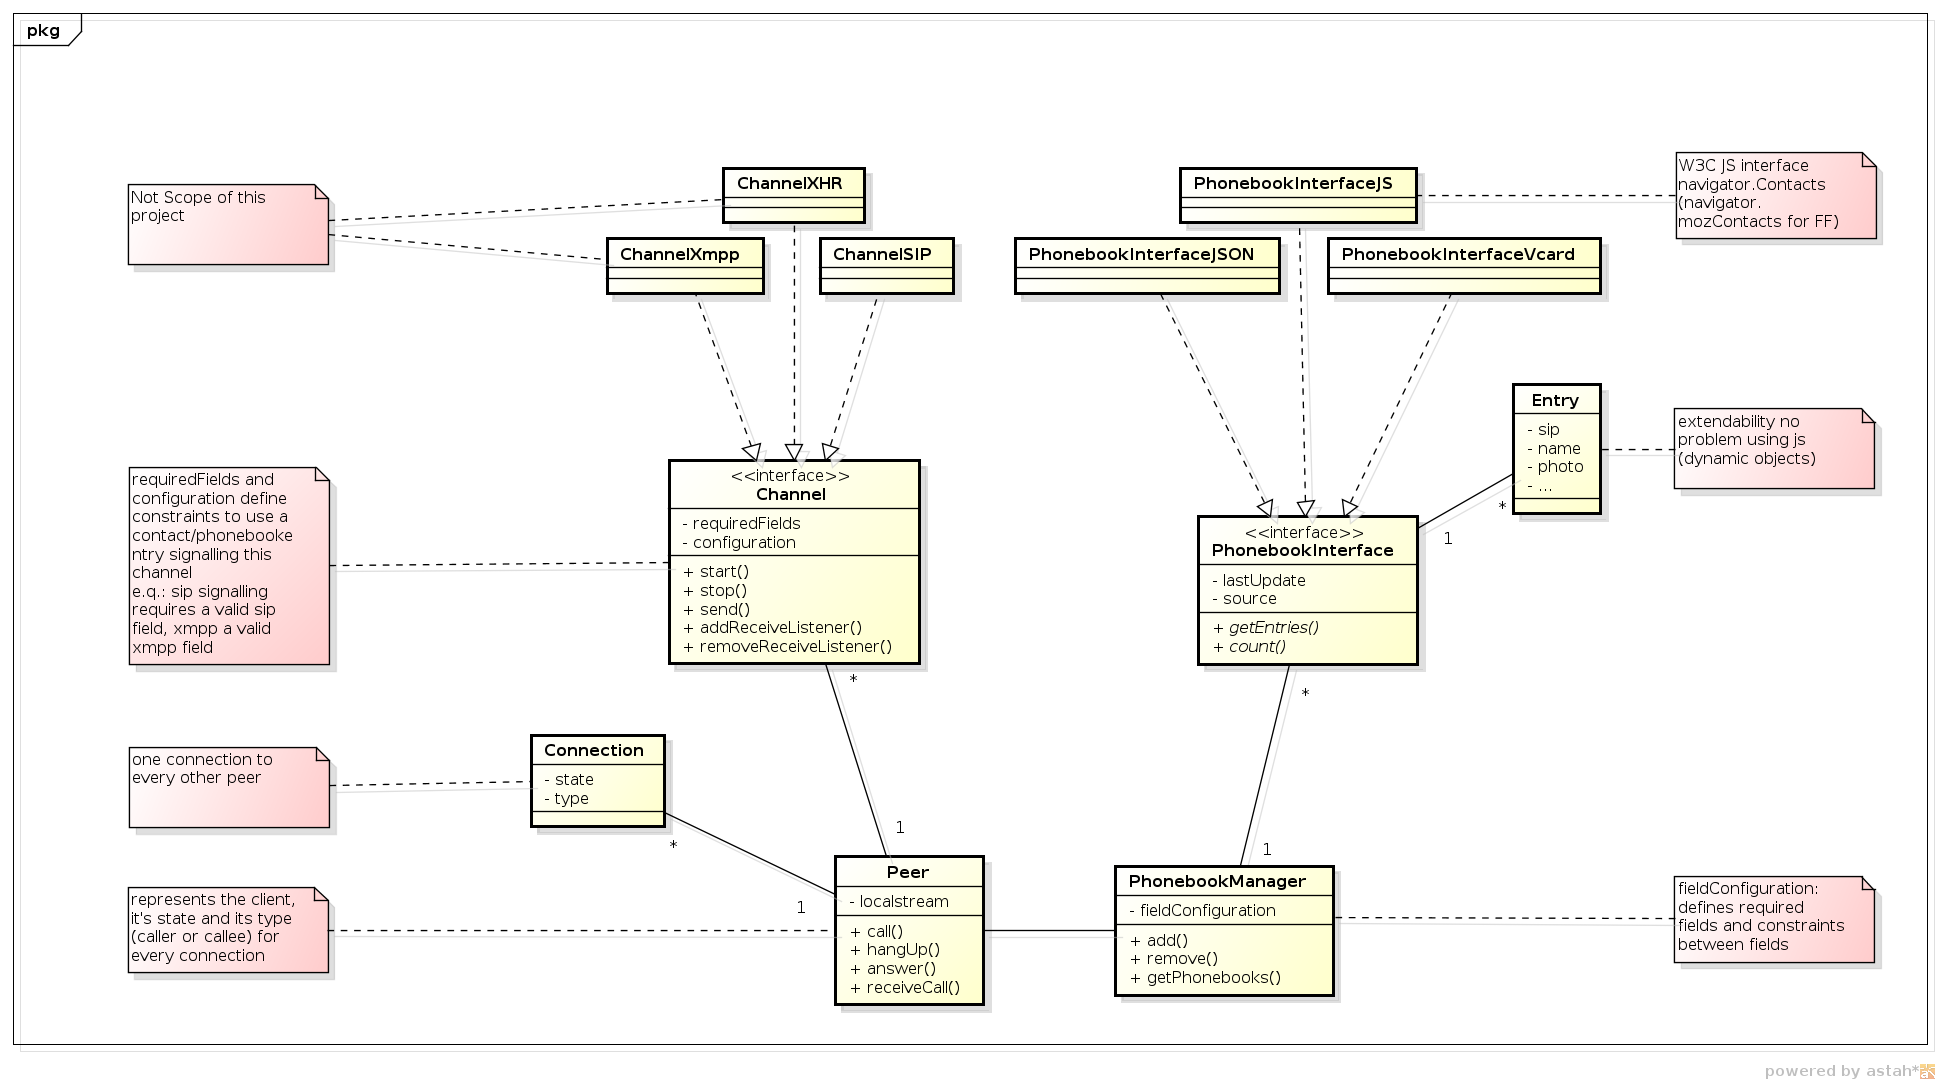
\includegraphics[width=1.2\textwidth]{../architekturanalayse/img/domain.png}
		%\caption{Strukturdiagramm JS VoIP App}
	\end{figure}
	Herzstück der Applikation sind die Channels und die Connection sowie das Contactbookmanagement.

\end{landscape}

\section{Channel}
	Die Channels laufen im Hintergrund und verbinden den User mit einem oder mehreren Signaling-Servern. Sie werden beim Login des Benutzers gestartet und müssen entsprechend ein Channel-Interface implementieren. So laufen z.B. ein SIP Channel und ein XHR Channel, ja nach dem was der Benutzer für Accounts besitzt.
	\begin{figure}[H]
		\centering
		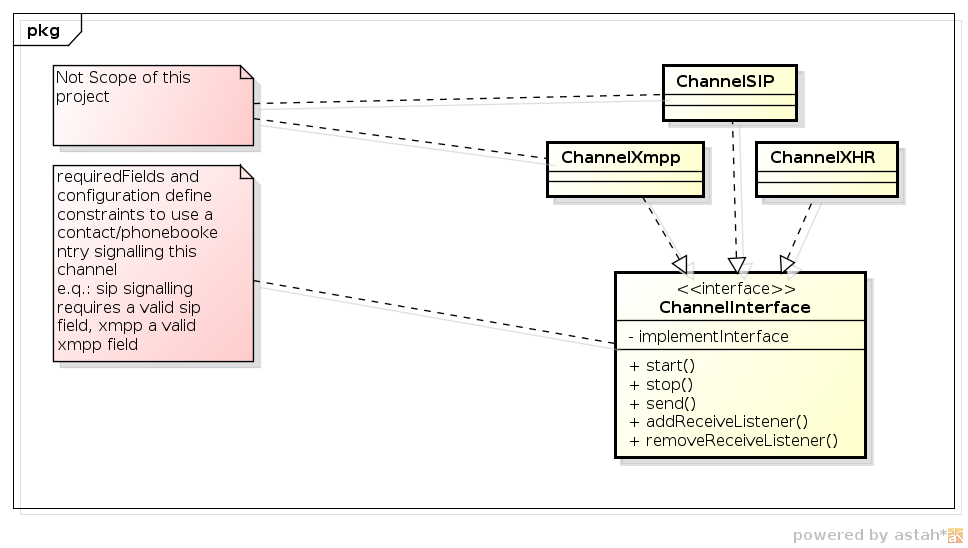
\includegraphics[width=\textwidth]{../architekturanalayse/img/channel.png}
		%\caption{Strukturdiagramm JS VoIP App}
	\end{figure}

\section{Adressbook}
	Die Kontaktverwaltung übernimmt der ContactbookManager. Er importiert Kontaktbücher anhand der Konfiguration von den Quelle "`Datei"', "`Ordner"' oder "`Online"'. Für die formatspezifischen Importprozesse sind die jeweiligen Kontaktbücher zuständig. Dazu müssen alle Kontaktbücher das Addressbook-Interface umsetzen.
	\begin{figure}[H]
		\centering
		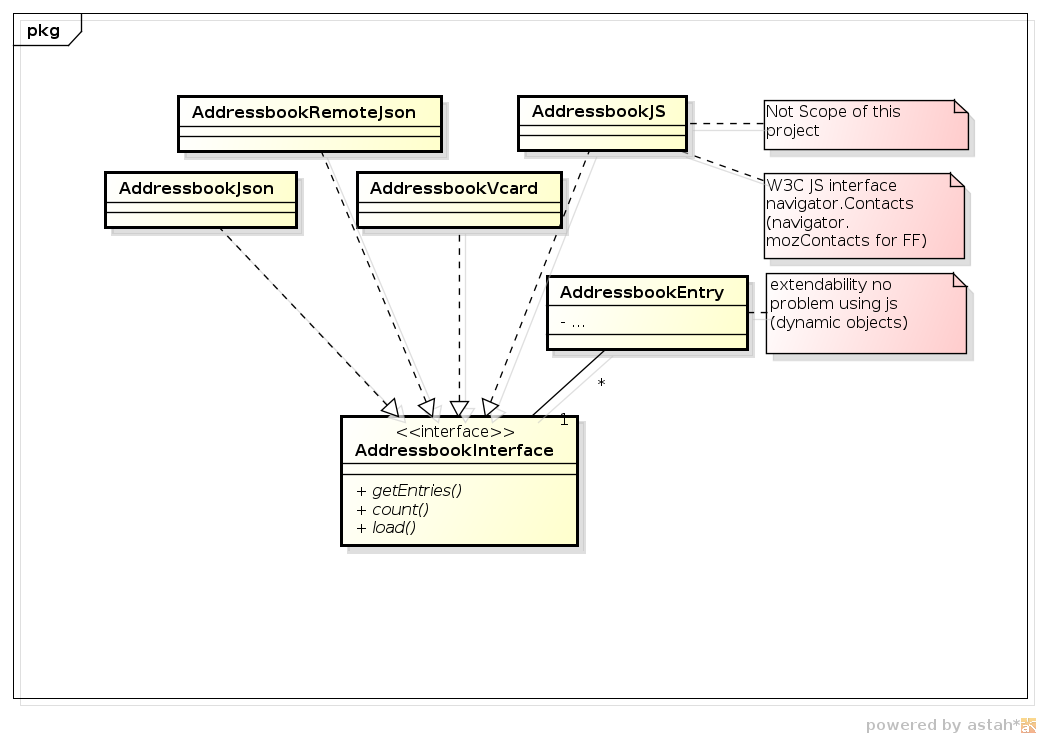
\includegraphics[width=\textwidth]{../architekturanalayse/img/addressbook.png}
		%\caption{Strukturdiagramm JS VoIP App}
	\end{figure}


\section{Interfaces}


\section{Connection}
	Die Connection übernimmt das komplette Handling der P2P-Verbindung inklusive Verbindungsauf- und -abbau. Sie greift über den Host auf die lokale Kamera zu und sendet und empfängt über einen Channel "`Offers"' und "`Answers/Replies"'.
	
	
	
	Die Kommunikation zwischen zwei Clients, einem STUN-Service und einem
	Signaling-Service wird im folgenden Diagramm dargestellt.
	\begin{figure}[H]
		\centering
		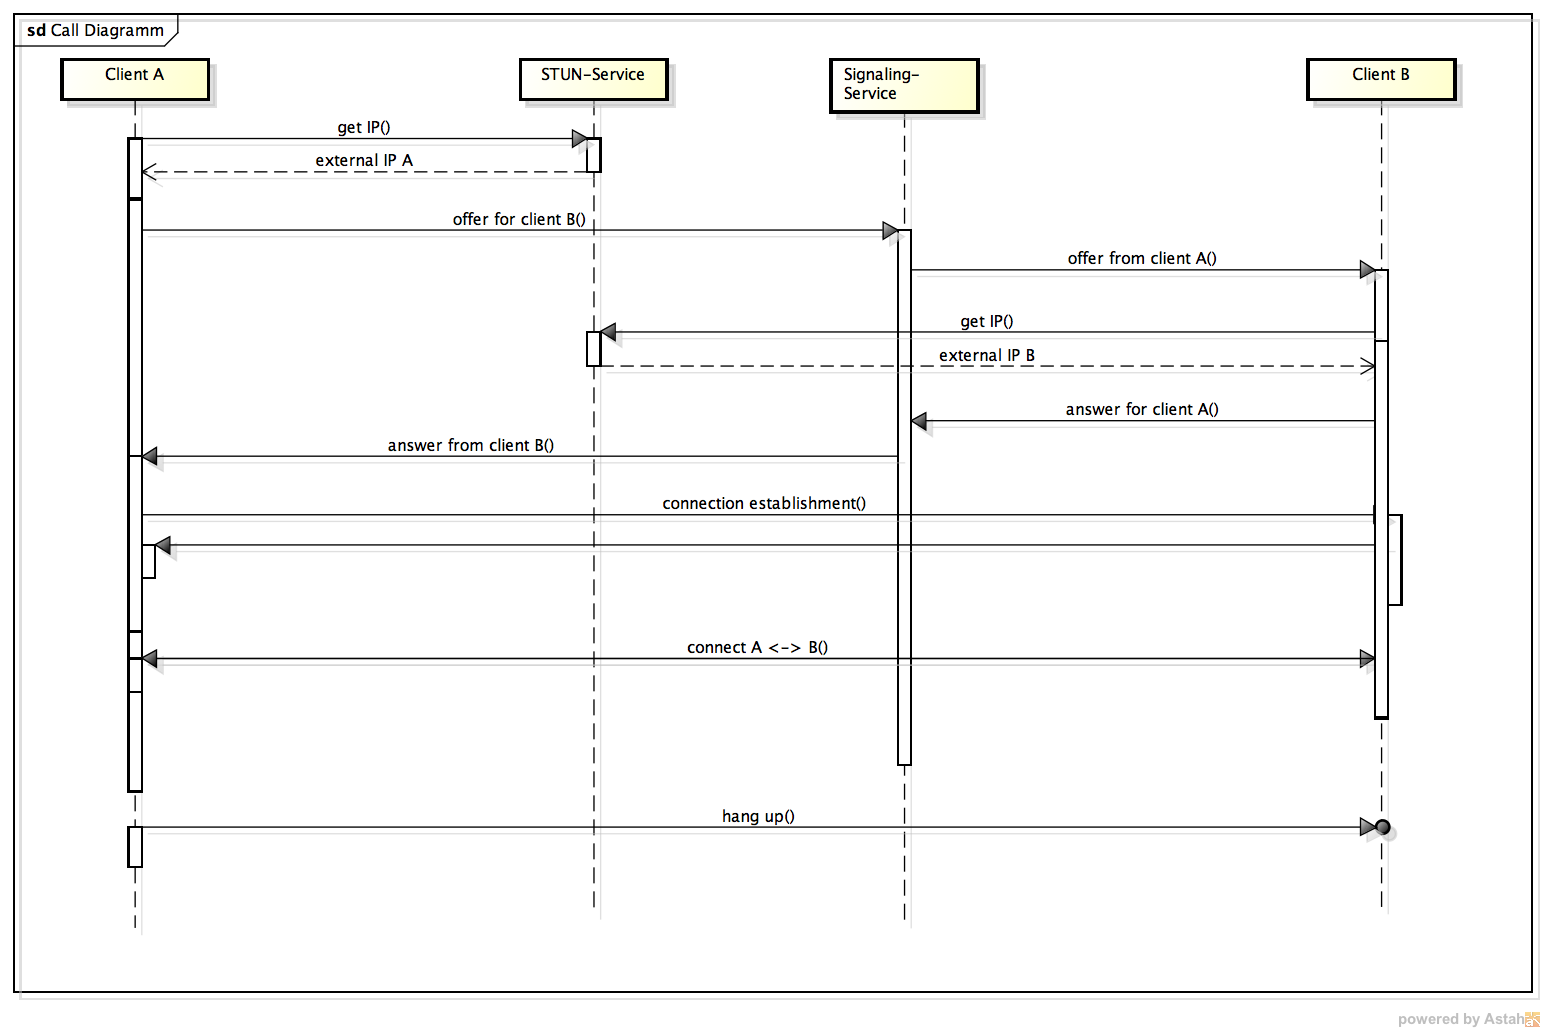
\includegraphics[width=\textwidth]{../architekturanalayse/img/callDiagramm.png}
		\label{img:deployment}
		\caption{Clientkommunikation}
	\end{figure}
	Die Clients beziehen vom STUN-Service ihre extern sichtbare IP und
	kommunizieren nach einem erfolgreichen Verbindungsaufbau direkt P2P ohne noch
	über den Signaling-Service zu gehen.
	
	Der Verbindungsabbau kann wahlweise über den Signaling-Server oder direkt P2P
	gesendet werden.
	
	
	\begin{landscape}		
		\begin{figure}[H]
			\centering
			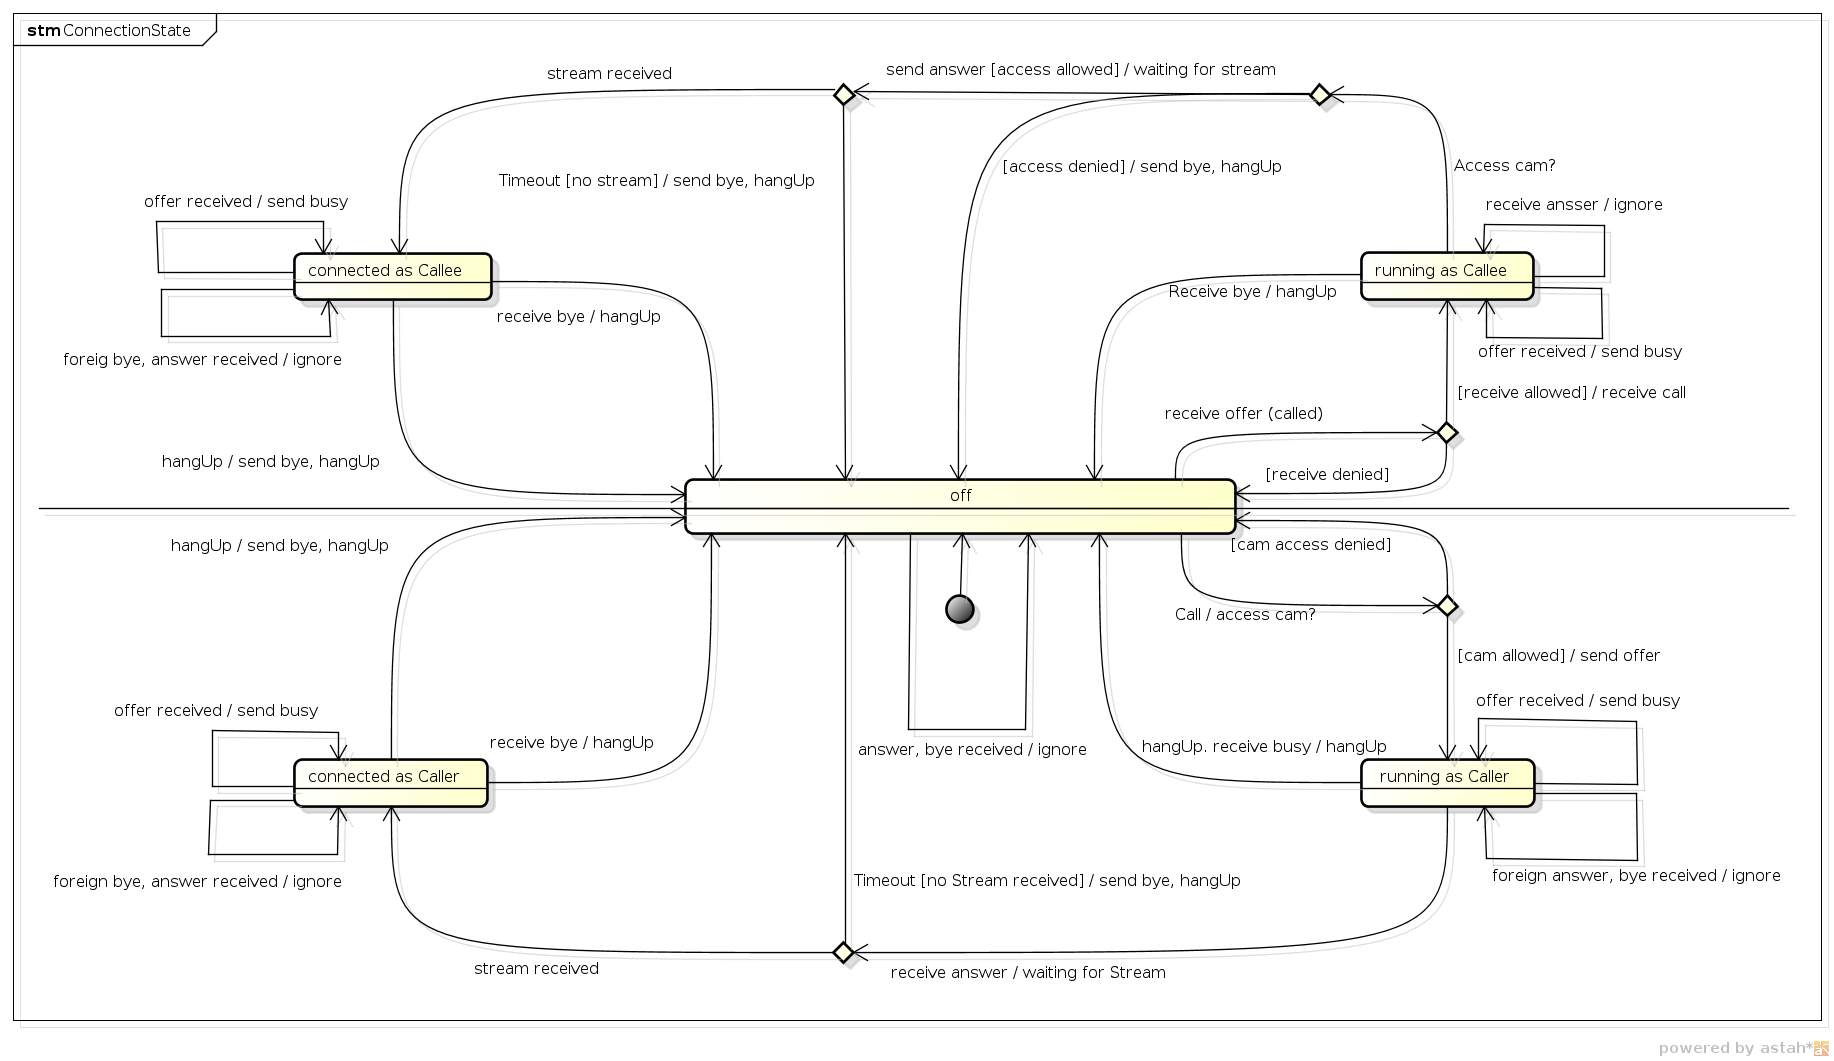
\includegraphics[height=0.7\textwidth]{../architekturanalayse/img/connectionState.png}
			\label{img:deployment}
			\caption{Applikationszustände}
		\end{figure}
		Beim Verbindungsaufbau nimmt jeder Client entwerde die Rolle "`Caller"' oder
		"`Callee"' ein. Erlaubt der Benutzer Zugriff auf die Kamera, so wird die
		Verbindung aufgebaut und bleibt bestehen, bis einer der Clients die Verbindung mit einem "`bye"' beendet.
		
		Ungültige Messages werden ignoriert. "`bye"' führt in jedem Zustand zu einem
		Abbruch der Verbindung bzw. des Aufbaus, vorausgesetzt das "`bye"'
		kommt vom anderen Kommunikationspartner.
	\end{landscape}
	


\clearpage

\section{Architektur-Designmotivations}

	\subsection{STUN-Service}
		STUN\footnote{Session Traversal Utilities for NAT \cite{IETF-STUN-RFC}}-Services sind zwingend
		notwendig, um die nach aussen sichtbare IP-Adresse des Clients herauszufinden.
		Neben der Möglichkeit, selbst einen STUN-Service aufzusetzen, gibt es frei
		verfügbare STUN-Services, beispielsweise von Mozilla oder Google.

		Für ein abgeschottetes Netz ist ein eigener STUN-Server zwingend notwendig.
		Für unseren Fall reichen die frei verfügbaren. Durch anpassen der
		Konfiguration ist es möglich, den Server festzulegen.

		Im Netz gibt es fertig konfigurierte virtuelle Maschinen mit einsatzbereitem
		STUN-Service\footnote{Mozilla, stun-vm \cite{Mozilla-STUN-VM}}.

	\subsection{SIP-Proxy vs. SIP-Server mit WebSockets}
		Unterstützt ein SIP-Server keine WebSockets, so kann ein SIP/WebSocket-Proxy
		dazwischen geschaltet werden. Die Konfiguration eines SIP-Proxies ist ähnlich
		aufwändig wie die Installation eines Kamailio
		\footnote{Kamailio SIP Server Project, \cite{Kamailio-Project}}-SIP-Servers, der in der neusten Version WebSockets unterstützt.

	\subsection{Sicherheit}
		WebRTC-Streams können nur verschlüsselt übertragen werden. Es gibt keine
		Möglichkeit, die Verschlüsselung abzuschalten. Dies führt zwar zu einem
		erhöhten Rechenbedarf auf dem Client, garantiert jedoch eine verschlüsselte
		Verbindung unabhängig von den Vorlieben des Entwicklers.
		Die Verschlüsselung erfolg über DTLS-SRTP\footnote{Datagram Transport Layer Security \cite{IETF-DTLS-RFC}} 
		keyings\footnote{Adam Roach, WebRTC: Security and Confidentiality \cite{AdamRoach-WebRTC-Security}}. 
		
		Die Verschlüsselung des Signaling-Channels ist abhängig von der eingesetzten
		Technologie. Werden z.B. Secure Websockets oder XHR über HTTPS eingesetzt so ist die Kommunikation verschlüsselt und nicht abgreifbar.
		
		Trotzdem kann ein Provider oder ein Geheimdienst Metadaten darüber sammeln, wer mit wem telefoniert.
		  
	\subsection{Hosting}
		Die JS-VoIP-App kann sowohl lokal, als auch von einem
		Webserver ausgeliefert ausgeführt werden. Es gibt keine speziellen Voraussetzungen. Ein Webserver ist daher nicht zwingend notwendig.
		